\section{Motivation}
\subsection{Compiler Optimizations}
In the past, researchers have shown that the choice of optimization sequences may impact software performance~\cite{almagor2004finding,chen2012deconstructing}. 
As a consequence, software-performance optimization becomes a key objective for both software industries and developers, which are often willing to pay additional costs to meet specific performance goals, especially for resource-constrained systems.

Universal and predefined sequences, \eg, O1 to O3 in GCC, may not always produce good performance results and may be highly dependent on the benchmark and the source code they have been tested on~\cite{hoste2008cole,chen2010evaluating,escobar2015evaluation}.
Indeed, each one of these optimizations interacts with the code and in turn with all other optimizations in complicated ways. Similarly, code transformations can either create or eliminate opportunities for other transformations and it is quite difficult for users to predict the effectiveness of optimizations on their source code program.
As a result, most software engineering programmers that are not familiar with compiler optimizations find difficulties to select effective optimization sequences~\cite{almagor2004finding}.

To explore the large optimization space, users have to evaluate the effect of optimizations according to a specific performance objective (see Figure 1). Performance can depend on different properties such as execution time, compilation time, resource consumption, code size, etc.
Thus, finding the optimal optimization combination for an input source code is a challenging and time-consuming problem. 
Many approaches~\cite{hoste2008cole,zhong2009tuning,sandran2012genetic,martins2014exploration} have attempted to solve this optimization selection problem using techniques such as Genetic Algorithms (GAs), machine learning techniques, etc.

%problem
It is important to notice that performing optimizations to source code can be so expensive at the expense of resource usage and may induce to compiler bugs or crashes. 
%With the increasing of resource usage, it is important to evaluate the compiler behavior. 
Indeed, in a resource-constrained environment and because of insufficient resources, compiler optimizations can even lead to memory leaks or execution crashes~\cite{yang2011finding}. 
Thus, a fine-grained understanding of resource consumption and analysis of compilers behavior regarding optimizations becomes necessary to ensure the efficiency of generated code.
\begin{figure}[h]
	\centering
	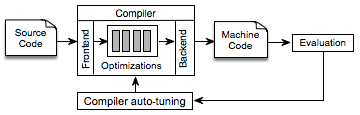
\includegraphics[width=0.9\linewidth]{Ressources/autotuning.png}
	\caption{Process of compiler optimizations exploration}
	
\end{figure}

\subsection{Example: GCC Compiler}

The GNU Compiler Collection, GCC, is a very popular collection of programming compilers, available for different platforms.
GCC exposes its various optimizations via a number of flags that can be turned on or off through command-line compiler switches. 
% We choose GCC compiler as a motivating example in order to explain how we would study the impact of compiler optimizations using a component-based infrastructure for testing and monitoring.
% In next section, we present a search-based technique called Novelty Search for automatic generation of optimization sequences.

For instance, version 4.8.4 provides a wide range of command-line options that can be enabled or disabled, including more than 150 options for optimization. The diversity of available optimization options makes the design space for optimization level very huge, increasing the need for heuristics to explore the search space of feasible optimization sequences.
For instance, we count 76 optimization flags that are enabled by the 4 default optimization levels (O1, O2, O3, Ofast). 
In fact, O1 reduces code size and execution time without performing any optimization that reduces the compilation time. It turns on 32 flags. 
O2 increases both compilation time and the performance of generated code. It turns on all optimization flags specified by O1 plus 35 other options. 
O3 is more aggressive level which enables all O2 options plus 8 more optimizations. 
Finally, Ofast is the most aggressive level which enables optimizations that are not valid for all standard-compliant programs. It turns on all O3 optimizations plus one more aggressive optimization. 
%For example, in GCC, we can distinguish optimization levels from O1 to O3. Each optimization level involves a fixed list of compiler optimization options
This results in a huge space with $2^{76}$ possible optimization combinations. The full list of optimizations is available here~\cite{mboussaa}.
%In our approach, we did not consider some optimization options that are enabled by default, since they do not affect the performance of generated binaries.
Optimization flags in GCC can be turned off by using \textit{"fno-"}+flag instead of \textit{"f"}+flag in the beginning of each optimization. 
We use this technique to play with compiler switches.
\iffalse
\begin{table}
	\label{table:options}
	\centering
	\caption{Compiler optimization options within standard optimization levels}
	\scalebox{0.88}{
		\begin{tabular}[c]{|c|p{3cm}||c|p{3cm}|}
			
			
			\cline{1-4}
			\textbf{Level} & \textbf{Optimization option} & \textbf{Level} & \textbf{Optimization option}  \\
			\hline
			O1 & 
			-fauto-inc-dec \newline
			-fcompare-elim \newline
			-fcprop-registers \newline
			-fdce \newline
			-fdefer-pop \newline
			-fdelayed-branch \newline
			-fdse \newline
			-fguess-branch-probability \newline
			-fif-conversion2 \newline
			-fif-conversion \newline
			-fipa-pure-const \newline
			-fipa-profile \newline
			-fipa-reference\newline 
			-fmerge-constants\newline 
			-fsplit-wide-types \newline
			-ftree-bit-ccp \newline
			-ftree-builtin-call-dce \newline
			-ftree-ccp \newline
			-ftree-ch \newline
			-ftree-copyrename \newline
			-ftree-dce \newline
			-ftree-dominator-opts \newline
			-ftree-dse \newline
			-ftree-forwprop \newline
			-ftree-fre \newline
			-ftree-phiprop \newline
			-ftree-slsr \newline
			-ftree-sra \newline
			-ftree-pta \newline
			-ftree-ter \newline
			-funit-at-a-time
			
			&
			\multirow{2}{*}{O2} & \multirow{2}{6cm} {
				-fthread-jumps\newline 
				-falign-functions\newline  
				-falign-jumps \newline
				-falign-loops  \newline
				-falign-labels \newline
				-fcaller-saves \newline
				-fcrossjumping \newline
				-fcse-follow-jumps  \newline
				-fcse-skip-blocks \newline
				-fdelete-null-pointer-checks \newline
				-fdevirtualize \newline
				-fexpensive-optimizations \newline
				-fgcse  \newline
				-fgcse-lm  \newline
				-fhoist-adjacent-loads \newline
				-finline-small-functions \newline
				-findirect-inlining \newline
				-fipa-sra \newline
				-foptimize-sibling-calls \newline
				-fpartial-inlining \newline
				-fpeephole2 \newline
				-fregmove \newline
				-freorder-blocks  \newline
				-freorder-functions \newline
				-frerun-cse-after-loop \newline 
				-fsched-interblock \newline 
				-fsched-spec \newline
				-fschedule-insns  \newline
				-fschedule-insns2 \newline
				-fstrict-aliasing \newline
				-fstrict-overflow \newline
				-ftree-switch-conversion\newline -ftree-tail-merge \newline
				-ftree-pre \newline
				-ftree-vrp
			} \\
			\cline{1-2}
			O3 & 
			-finline-functions \newline
			-funswitch-loops\newline
			-fpredictive-commoning \newline
			-fgcse-after-reload \newline
			-ftree-vectorize \newline
			-fvect-cost-model \newline
			-ftree-partial-pre \newline 
			-fipa-cp-clone  & &  \\
			\cline{1-2}
			Ofast & -ffast-math &   &  \\
			\hline
			
		\end{tabular}
	}
\end{table}
\fi